%%%%%%%%%%%%%%%%%%%%%%%%%%%%% Define Article %%%%%%%%%%%%%%%%%%%%%%%%%%%%%%%%%%
\documentclass{article}
%%%%%%%%%%%%%%%%%%%%%%%%%%%%%%%%%%%%%%%%%%%%%%%%%%%%%%%%%%%%%%%%%%%%%%%%%%%%%%%

%%%%%%%%%%%%%%%%%%%%%%%%%%%%% Using Packages %%%%%%%%%%%%%%%%%%%%%%%%%%%%%%%%%%
\usepackage[utf8]{inputenc}
\usepackage{float, geometry, graphicx, fancyhdr, color, xcolor}
\usepackage{amssymb, amsthm, amsmath, tikz, pgfplots, comment, wrapfig}
\usepackage{listings, mdframed, lipsum, psfrag, parskip, empheq, subfig, verbatim, pythonhighlight}
\usepackage[english]{babel}
\usepackage[breaklinks]{hyperref}
\usepackage{titlesec, cite, hyperref, wrapfig, booktabs, bookmark, pdfpages, lastpage}
\usepackage{upgreek}

%%%%%%%%%%%%%%%%%%%%%%%%%%%%%%%%%%%%%%%%%%%%%%%%%%%%%%%%%%%%%%%%%%%%%%%%%%%%%%%

%%%%%%%%%%%%%%%%%%%%%%%%%% C Code Listing Settings %%%%%%%%%%%%%%%%%%%%%%%%%%%%%%%%%%%%%%%
\definecolor{mGreen}{rgb}{0.25,0.63,0.15}
\definecolor{mGray}{rgb}{0.5,0.5,0.5}
\definecolor{mPurple}{rgb}{0.58,0,0.82}
\definecolor{codeBlue}{rgb}{0.01, 0.2, 0.92}
\definecolor{codegray}{rgb}{0.5,0.5,0.5}
\definecolor{codepurple}{rgb}{0.58,0,0.82}
\definecolor{codeblue}{rgb}{0.13,0.29,0.53}
\definecolor{backgroundColour}{rgb}{0.95,0.95,0.95}

\lstset{
    language=Python,
    backgroundcolor=\color{backgroundColour},
    basicstyle=\ttfamily\small,
    commentstyle=\color{deepGreen},
    keywordstyle=\color{blue},
    numberstyle=\tiny\color{mGray},
    stringstyle=\color{red},
    breakatwhitespace=false,         
    breaklines=true,                 
    captionpos=b,                    
    keepspaces=true,                 
    numbers=left,                    
    numbersep=5pt,                  
    showspaces=false,                
    showstringspaces=false,
    showtabs=false,                  
    tabsize=2,
    frame=single
}

%%%%%%%%%%%%%%%%%%%%%%%%%%%%%%%%%%%%%%%%%%%%%%%%%%%%%%%%%%%%%%%%%%%%%%%%%%%%%%%

% Other Settings
\hypersetup{
    colorlinks = true,
    linkcolor = black,
    urlcolor = blue,
}
\urlstyle{same}

%%%%%%%%%%%%%%%%%%%%%%%%%% Page Setting %%%%%%%%%%%%%%%%%%%%%%%%%%%%%%%%%%%%%%%
\geometry{a4paper}
\pagestyle{fancy}
\fancyhead{}
\fancyhead[L]{Computational Intelligence}
\fancyhead[C]{Assignment 02 - Report}
\fancyhead[R]{CS 451}
\fancyfoot{}
\fancyfoot[C]{\thepage \;of \pageref{LastPage}}

%%%%%%%%%%%%%%%%%%%%%%%%%% Define some useful colors %%%%%%%%%%%%%%%%%%%%%%%%%%
\definecolor{ocre}{RGB}{243,102,25}
\definecolor{mygray}{RGB}{243,243,244}
\definecolor{deepGreen}{RGB}{26,111,0}
\definecolor{shallowGreen}{RGB}{235,255,255}
\definecolor{deepBlue}{RGB}{61,124,222}
\definecolor{shallowBlue}{RGB}{235,249,255}
%%%%%%%%%%%%%%%%%%%%%%%%%%%%%%%%%%%%%%%%%%%%%%%%%%%%%%%%%%%%%%%%%%%%%%%%%%%%%%%

%%%%%%%%%%%%%%%%%%%%%%%%%% Define an orangebox command %%%%%%%%%%%%%%%%%%%%%%%%
\newcommand\orangebox[1]{\fcolorbox{ocre}{mygray}{\hspace{1em}#1\hspace{1em}}}
%%%%%%%%%%%%%%%%%%%%%%%%%%%%%%%%%%%%%%%%%%%%%%%%%%%%%%%%%%%%%%%%%%%%%%%%%%%%%%%

%%%%%%%%%%%%%%%%%%%%%%%%%%%% English Environments %%%%%%%%%%%%%%%%%%%%%%%%%%%%%
\newtheoremstyle{mytheoremstyle}{3pt}{3pt}{\normalfont}{0cm}{\rmfamily\bfseries}{}{1em}{{\color{black}\thmname{#1}~\thmnumber{#2}}\thmnote{\,--\,#3}}
\newtheoremstyle{myproblemstyle}{3pt}{3pt}{\normalfont}{0cm}{\rmfamily\bfseries}{}{1em}{{\color{black}\thmname{#1}~\thmnumber{#2}}\thmnote{\,--\,#3}}
\theoremstyle{mytheoremstyle}
\newmdtheoremenv[linewidth=1pt,backgroundcolor=shallowGreen,linecolor=deepGreen,leftmargin=0pt,innerleftmargin=20pt,innerrightmargin=20pt,]{theorem}{Theorem}[section]
\theoremstyle{mytheoremstyle}
\newmdtheoremenv[linewidth=1pt,backgroundcolor=shallowBlue,linecolor=deepBlue,leftmargin=0pt,innerleftmargin=20pt,innerrightmargin=20pt,]{definition}{Definition}[section]
\theoremstyle{myproblemstyle}
\newmdtheoremenv[linecolor=black,leftmargin=0pt,innerleftmargin=10pt,innerrightmargin=10pt,]{problem}{Problem}[section]
%%%%%%%%%%%%%%%%%%%%%%%%%%%%%%%%%%%%%%%%%%%%%%%%%%%%%%%%%%%%%%%%%%%%%%%%%%%%%%%


\title{{\huge \textbf{Habib University \\ Computational Intelligence - CS 451}}

\vspace*{5mm}
{\LARGE \textbf{Assignment 02 - Report} \\ \textbf{Swarm Intelligence}}
{
\includegraphics[width=0.75\linewidth]{logo.png}} \\ 
{\Large \textbf{Instructor:} Dr. Saleha Raza}}
\author{Ali Muhammad Asad - aa07190 \\ Dua Batool - db07098}
\date{}

\pgfplotsset{compat=1.18}

\begin{document}
\maketitle

\newpage
\tableofcontents

\newpage
\section{Question 1 - Graph Coloring Problem using Ant Colony Optimization}
\subsection{Introduction and Problem Formulation}
The Graph Coloring Problem is a well known problem in Computer Science that asks a really simple question, "What is the minimum number of colors required to color a graph such that no two adjacent vertices have the same color?". This problem is NP-Hard, a combinatorial optimization problem, and has a lot of real world applications. The image below shows a graph and its corresponding coloring.
\begin{figure}[htbp]
    \centering
    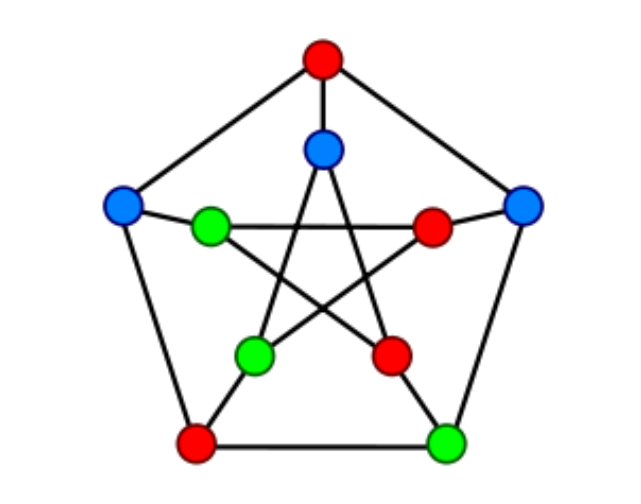
\includegraphics[width=0.35\textwidth]{../gco.png}
    \caption{Graph Coloring Example}
\end{figure}

In this assignment, the Ant Colony Optimization (ACO) Algorithm is used to efficiently provide a solution for coloring of a graph with minimum number of colors. The ACO algorithm is a probabilistic technique for solving computational problems which can be reduced to finding good paths through graphs. The ACO algorithm is inspired by the foraging behavior of ants and is a class of optimization algorithms that are based on the behavior of ants.

The problem can be formally formulated as follows:
\begin{definition}
    Given a graph $G = (V, E)$, where $V$ is the set of vertices and $E$ is the set of edges, a $k$-coloring of $G$ is a mapping such that $c: V \to \{ 1, 2, 3, ..., k \} $ is a mapping from the set of vertices to the set of colors such that $ \forall u, v \in V, \{ u, v \} \in E $ where $ \{u, v\} $ represents an edge from vertex $u$ to vertex $v$, $c(u) \neq c(v)$. The objective is to find the minimum value of $k$ such that a $k$-coloring of $G$ exists.
\end{definition}

We invoke the help of a theorem in Graph Theory for our implementation which makes things much easier for us, and helps us get to the solution faster. The theorem is as follows:
\begin{theorem}
    If $G$ is a simple graph with the largest vertex degree $ \triangle $, then $G$ is $ (\triangle + 1) $-colorable.
\end{theorem}
The above theorem is used in the color assignments, due to which the color assignement is initially sub-optimal, and not equal to the number of nodes, thus we get to an optimal solution much faster.

\subsection{Ant Colony Optimization and Graph Coloring}
\textbf{Ant Colony Optimization (ACO)} is a probabilistic technique inspired by the food foraging behavior of ants, seeking a path between their colony and a food source. The algorithm is characterized by the collective behavior of simple agents (ants) communicating indirectly via pheromone trails, which leads to the emergence of intelligent global behavior.

\begin{figure}[htbp]
    \centering
    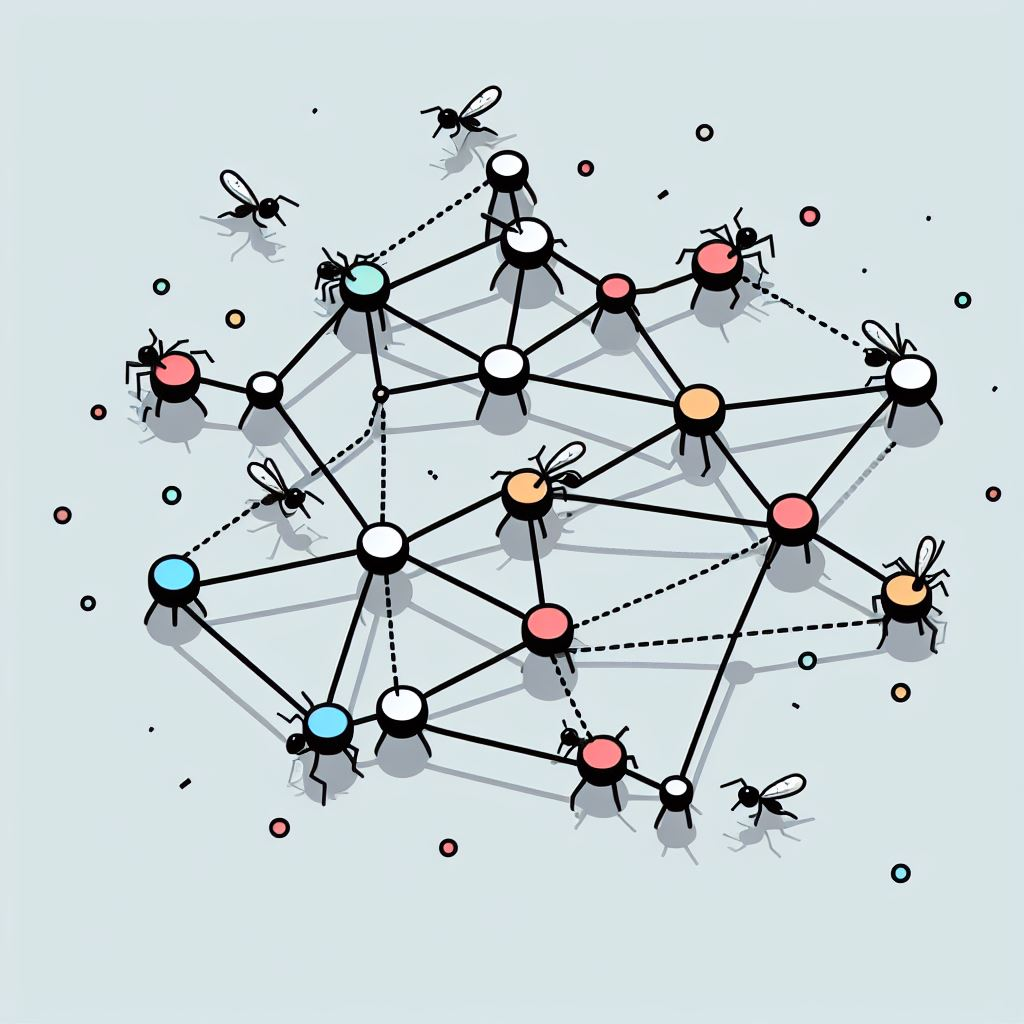
\includegraphics[width=0.45\textwidth]{antcol.jpeg}
    \caption{Some ants on a graph}
\end{figure}

\textbf{Graph Coloring} can be solved by applying ACO by considering the following steps:
\begin{enumerate}
    \item \textbf{Initialization:} Each ant, which represents a potential solution, is placed on a random vertex of the graph.The ants will traverse the graph, visiting each vertex exactly once and assigning it a color. The goal is to use as few colors as possible while ensuring that no two adjacent vertices share the same color.
    \item \textbf{Color Assignment:} When an ant visits a vertex, it assigns a color to that vertex. The color is chosen based on a probabilistic rule that takes into account the amount of pheromone associated with each color and the visibility (a heuristic information). The visibility can be defined in various ways, for example, as the number of uncolored neighbors of the current vertex.
    \item \textbf{Pheromone Update:} After all ants have constructed their solutions (i.e., colored the graph), the pheromone trails are updated. More pheromone is deposited on the color assignments that led to better solutions (i.e., colorings that used fewer colors). This guides future ants towards these better solutions.
    \item \textbf{Evaporation:} To avoid premature convergence and to encourage exploration, some amount of pheromone evaporates after each iteration. This reduces the influence of earlier solutions and allows for the possibility of finding better solutions.
    \item \textbf{Iterations:} The process of ants constructing solutions and updating pheromone trails is repeated for a number of iterations. Over time, the algorithm converges towards an optimal or near-optimal solution.
\end{enumerate}

% \subsection{Implementation of the Ant Colony Optimization Algorithm}
% The implementation of the ACO algorithm for the Graph Coloring Problem is mainly done using three separate classes, namely the \texttt{Graph}, \texttt{Cheenti}, and \texttt{GraphColorACO} classes. The \texttt{Graph} class is used to represent the graph structure, the \texttt{Cheenti} class is used to represent an ant which acts as our artificial agent, and the \texttt{GraphColorACO} class is used to represent the Ant Colony that solves the Graph Coloring Problem.
\subsection{Graph Representation}
This class basically handles loading the graph from a file, and then creating the graph structure. The graph is implemented as a dictionary, where each key represents a node, and the corresponding value is a set of its neighboring nodes. The value associated with each key is specifically chosen to be a \pyth{set} for easier operations such as union, intersection, and difference. This representation is suited for an undirected graph, as an edge between nodes $u$ and $v$ implies an edge between $v$ and $u$.

The \pyth{Graph} class includes the following methods:
\begin{itemize}
    \item The \pyth{neighbors()} method returns the neighbors of a given node and also in a given set of nodes (passed as arguments). This is particularly useful for exploring unvisited nodes in the graph while an ant traverses the graph.
    \item The \pyth{degreesSingleNode()} method returns the degree of a given node, which is the number of edges incident to the node.
    \item The \pyth{degreesPlus()} method returns the degree of a given node, that are also in a \pyth{set} provided as argument, which is useful for calculating the visibility of a node.
\end{itemize}

\subsection{Ant Colony and the Ant Representation}
An ant - artificial agent - is represented as a class \pyth{Cheenti}. Each ant has several attributes and methods that help it traverse the graph, calculate probabilities, visibility / desirability of a node, and update the pheromone matrix. Thus, each ant is responsible for constructing a solution to the Graph Coloring Problem. For our implementation, mainly the ``Recursive Largest First'' \hyperlink{refpaper}{[1]}\hyperlink{rlfmethod}{[2]} method has been used, where classes of colors are built sequentially. Once a vertex $v \in V$, where $V$ is the set of vertices have not been colored yet, such that the maximum degree of $V$is deg$_V(v)$ has been selected, the current stable is augmented by inserting as long as possible the vertex $ v \in V \cap U $ with maximum degree deg$_U(v)$ where the set $U$ contains every uncolored vertex, which cannot belong to the stable under construction \hyperlink{refpaper}{[1]}.

An instance of an \pyth{Ant} is initialized with the following parameters and has the following attributes as well:
\begin{itemize}
    \item \pyth{alpha} which is the relative importance of the pheromone trail,
    \item \pyth{beta} which is the relative importance of the visibility of a node,
    \item \pyth{Q} which is the amount of pheromone deposited by the ant,
    \item \pyth{graph} which is the graph to be colored,
    \item \pyth{colors} which is the list of colors available to the ant,
    \item \pyth{distance} which is the total distance of the path traversed by the ant
    \item \pyth{colorMap}, and \pyth{colorAssign}, which are dictionaries that map nodes to colors.
\end{itemize}

The \pyth{initializeColors()} method intializes the color map and color assignment dictionaries for each node in the graph. The color map is a dictionary where each key is a color, and the value is a set of nodes colored with that color. The color assignment is a dictionary where each key is a node, and the value is the color assigned to that node. Two separate dictionaries were used to make the implementation easier and more efficient. The color map dictionary maps each color to the set of nodes that are assigned that color. It's used to keep track of which nodes have been assigned which color. This is useful for quickly finding all nodes of a particular color, such as in getting pheromone trails, and finding if a color is not already mapped to a node while traversing the graph. The color assignment dictionary maps each node to the color that it has been assigned. It's used to keep track of the current color of each node. This is useful for quickly checking or updating the color of a specific node, and also in updating the pheromone matrix locally for an ant.

% \vspace*{2mm}
% \textbf{Updating the Pheromone Trails}
\subsubsection{Updating the Pheromone Trails}

In our implementation, pheromone trails are related to pairs of nonadjecant vertices. So each pair of nodes $ (v_i, v_j) $ has an associated pheromone trail $ \uptau(v_i, v_j) $ where the vertex $ v_i $ and $ v_j $ have the same color. The pheromone trails are updated after each ant has constructed a solution. The pheromone trails are updated based on the quality of the solution. More pheromone is deposited on the color assignments that led to better solutions (i.e., colorings that used fewer colors). This guides future ants towards these better solutions. For ease of implementation, the pheromone trails are stored in a matrix of order $n \times n$ where $n$ is the number of nodes in the graph. This represents an adjacency matrix, which makes it easier to update the pheromone trails for each pair of nodes.

Values of pheromones are associated to pairs of nonadjecant vertices having the same color. Formally, the value $ \uptau^k(v_i, v_j) $ corresponds to the trace left by a given ant $k$ having assigned the same color to vertices $ v_i $ and $ v_j $ where $ (1 \leq i \neq j \leq n) $. Therfore, at the end of a cycle of the algorith, $ \uptau(v_i, v_j) $ is the value of pheromone associated to the couple $ (v_, v_j) $ for all colorings (ants) which colored $ v_i $ and $ v_j $ with the same color \hyperlink{refpaper}{[1]}. One ant calculates its own local pheromone trail, which is then updated in a global pheromone matrix. Initially, the pheromones are set to 1, and as the ants traverse the graph, the values for pheromones between any two nodes an ant visits is simply the value $Q$ which is the amount of pheromones an ant deposits. However, since we have an evaporation rate, in each iteration, the pheromones are simply updated by multiplying them by a factor of $ (1 - \upgamma) $ where $ \upgamma $ is the evaporation rate.

Thus, their initialization is defined as:
\[
    \text{\Large $\uptau(v_i, v_j) = $ }
    \begin{cases}
        1 & (v_i, v_j) \in E    \\
        0 & (v_i, v_j) \notin E
    \end{cases}
\]
and their stage by stage update for each $k$th ant is defined as:
\[ \forall(v_i, v_j) \in S_k: \uptau(v_i, v_j) = (1 - \upgamma) * \uptau(v_i, v_j) + \upgamma * \uptau_0 \]
and evaporation is carried out according to the rule:
\[ \uptau(v_i, v_j) = (1 - \upgamma) * \uptau(v_i, v_j) \]
where $ S_k $ is the solution built by the $k$th ant, $ \upgamma \in [0, 1] $ pheromone trails persistance, $ \upgamma $ is the evaporation rate, and $ \uptau_0 $ is the initial value of the pheromone \hyperlink{refpaper}{[1]}. The pheromone trails are updated after each ant has constructed a solution. The pheromone trails are updated based on the quality of the solution. More pheromone is deposited on the color assignments that led to better solutions (i.e., colorings that used fewer colors). This guides future ants towards these better solutions.

% \vspace*{2mm}
% \textbf{Heuristic Information}
\subsubsection{Heuristic Information}

As mentioned in the reference paper \hyperlink{refpaper}{[1]}, ants are implemented as RLF, then heuristic information $ \upeta(v_i, v_j) $, relative to the choice of the vertex $v_j$, starting from the current vertex $ v_i $ is defined in three possible ways:
\begin{align}
    \upeta(v_i, v_j) & = \text{deg}_B(v_j)               \\
    \upeta(v_i, v_j) & = \mid A \mid - \text{deg}_A(v_j) \\
    \upeta(v_i, v_j) & = \text{deg}_{A \cup B}(v_j)
\end{align}
where $A$ is the set of nodes that have not been visited, and thus have not been colored, and $B$ is the set of nodes that have been visited, and thus have been colored. The first method is the number of uncolored neighbors of the current vertex, the second method is the number of uncolored neighbors of the current vertex, and the third method is the number of uncolored neighbors of the current vertex. This visibility / desirability is used to calculate the probability of an ant choosing a particular node to visit next. After trial and error, the first method was chosen for our implementation, as it gave the best results.

% \vspace*{2mm}
% \textbf{Transition Rule}
\subsubsection{Transition Rule}

The above visibility / desirability is then used to compute the probabilities of an ant choosing a particular node to visit next. In this implementation, more importance is given to information collected by previous ants, with respect to the exploration of the search space \hyperlink{refpaper}{[1]}. This is achieved using two mechanisms. First, a strong elitist strategy is used to update the pheromone trails, and second, ants choose the next vertex $v$ to move to (and thus color) applying a pseudo-random proportional rule: with probability $ q_0 $, they move to the vertex $j$ for which the product between the pheromone trail and heuristic information is maximum. That is, $ v = \text{max}\{ (\uptau)^\alpha(t) \times (\upeta_{ij})^\beta (t) \} $, while with probability $ 1 - q_0 $ they operate a biased exploration in which the probability $ p_{ij}^k(t) $ is given by:
\[
    P_{ij}^k (t) = \displaystyle\frac{(\uptau_{ij})^\alpha(t) \times (\upeta_{ij})^\beta(t)}{\displaystyle\sum_{l \in N_i^k}(\uptau_{il})^\alpha (t) \times (\upeta_{il})^\beta (t)}
\]
where $ \uptau_{ij} $ is the value of the pheromone on edge $(i, j)$ at the $t$-th iteration, and $ \upeta_{ij}(t) $ the heuristic information associated to the vertex $j$ at the $t$-th iteration, and $ N_i^k $ is the feasible neighborhood of ant $k$ - the set of vertices which the ant has not yet visited\hyperlink{refpaper}{[1]}.


\subsection{Results and Analysis}
\subsubsection{Parameter Values}
After trial and error, the following paramter values were set for the ACO algorithm:
\begin{itemize}
    \item \pyth{alpha} = 4.0
    \item \pyth{beta} = 4.0
    \item \pyth{gamma} = 0.9
    \item \pyth{Q} = 10
    \item \pyth{numAnts} = 20
    \item \pyth{Iterations} = 100
\end{itemize}

\subsubsection{Heuristic Selection}
We decided to use heuristics 1 and 3 for the visibility / desirability of a node. Some of the computations with the above mentioned parameters, with all three heuristics are shown below.

\textbf{Heuristic 1 $ (\upeta(v_i, v_j)) = \text{deg}_B(v_j) $}
\begin{figure}[H]
    \centering
    \begin{tabular}{| c | c |}
        \hline
        \subfloat[Dataset 1, Queen11]{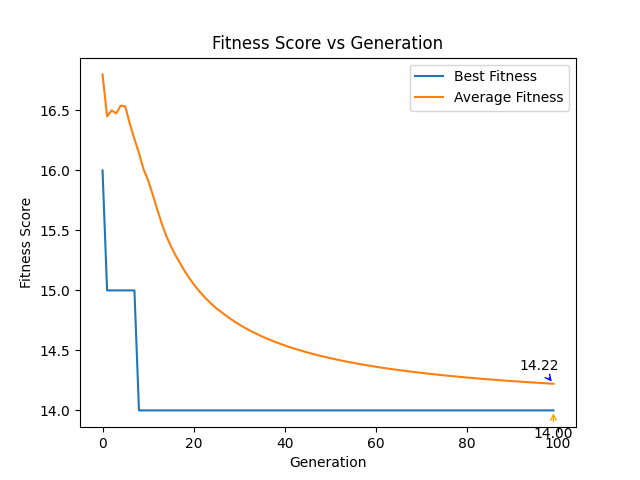
\includegraphics[width=0.475\textwidth]{../report/results/GCO_d1_1.png}} & \subfloat[Dataset 2, le450]{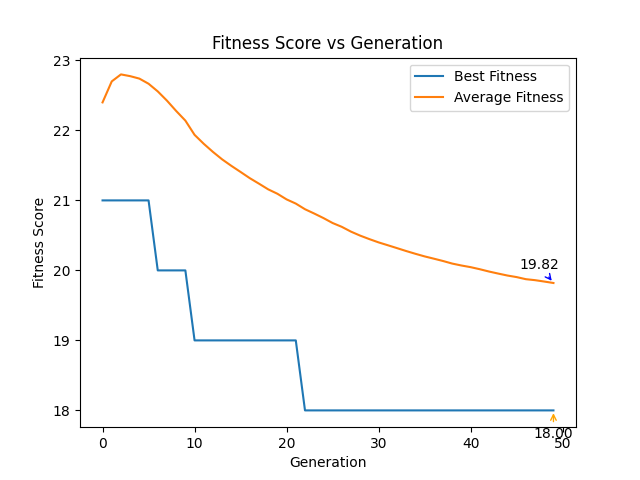
\includegraphics[width=0.475\textwidth]{../report/results/GCO_d2.png}} \\ \hline
    \end{tabular}
    \caption{Results using Heuristic 1}
\end{figure}

We can see a good optimization in the best solution, and the average solution as well. The average solution is going towards a convergence, and the best solution is also getting better.

\textbf{Heuristic 2 $ \upeta(v_i, v_j) = \mid A \mid - \text{deg}_A(v_j) $}

\begin{figure}[H]
    \centering
    \begin{tabular}{| c | c |}
        \hline
        \subfloat[Dataset 1, Queen11]{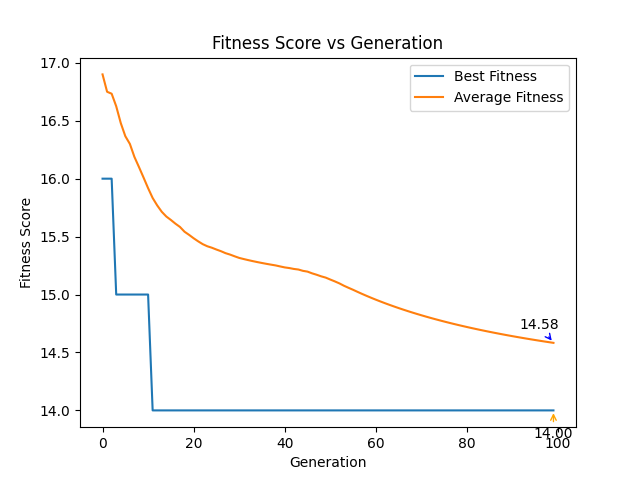
\includegraphics[width=0.475\textwidth]{../report/results/GCO_d1_h2_1.png}} & \subfloat[Dataset 2, le450]{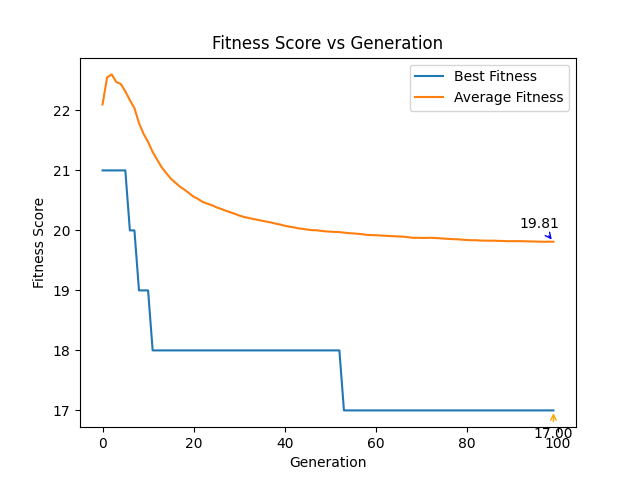
\includegraphics[width=0.475\textwidth]{../report/results/GCO_d2_h2.png}} \\ \hline
    \end{tabular}
    \caption{Results using Heuristic 2}
\end{figure}

Although there is still some optimization, the results are not as good as the ones with heuristic 1. The average solution is converging much slower, and we see in dataset 2 it is almost approaching a horizontal line without even converging towards the best solution.

\textbf{Heuristic 3 $ \upeta(v_i, v_j) = \text{deg}_{A \cup B}(v_j) $}

\begin{figure}[H]
    \centering
    \begin{tabular}{| c | c |}
        \hline
        \subfloat[Dataset 1, Queen11]{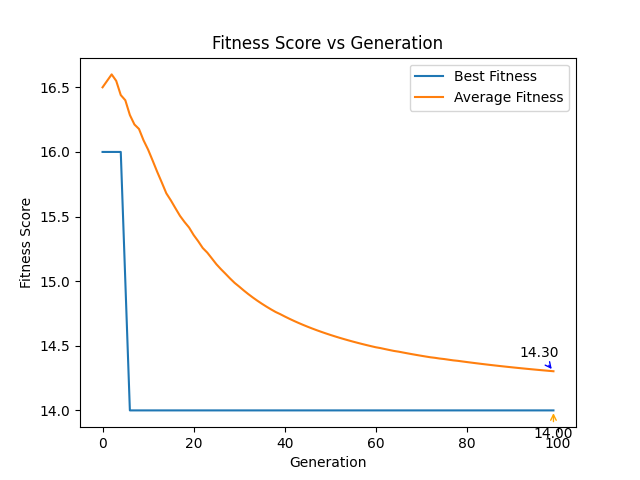
\includegraphics[width=0.475\textwidth]{../report/results/GCO_d1_h3.png}} & \subfloat[Dataset 2, le450]{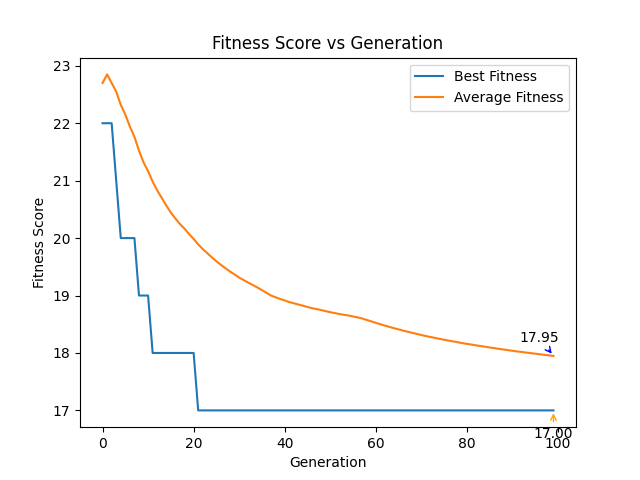
\includegraphics[width=0.475\textwidth]{../report/results/GCO_d2_h3_best.png}} \\ \hline
    \end{tabular}
    \caption{Results using Heuristic 3}
\end{figure}

We can see that heuristic 3 is also really good, especially for the dataset 2. The average solution is converging towards the best solution, and the best solution is also getting better. The results are almost as good as the ones with heuristic 1 for dataset 1, but better for dataset 2.

\subsubsection{Parameter Sensitivity}

The values for the parameters were found after various trial and error. Some of them are shown below as well.

\textbf{Alpha is lower than Beta}
\begin{figure}[H]
    \centering
    \begin{tabular}{| c | c |}
        \hline
        \subfloat[Dataset 1, Queen11]{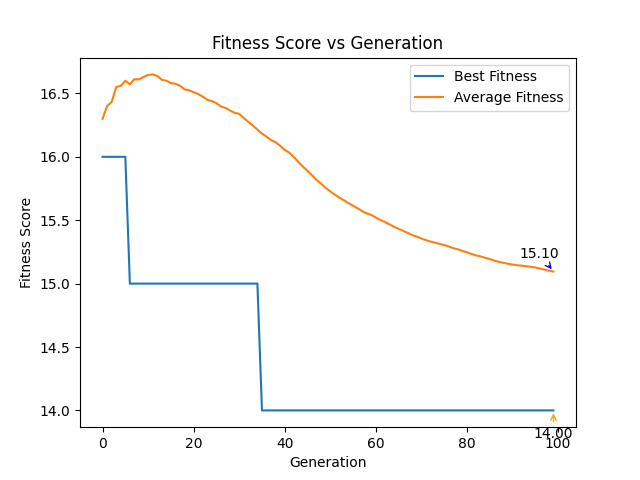
\includegraphics[width=0.475\textwidth]{../report/results/GCO_d1_a2_b4_use.png}} & \subfloat[Dataset 2, le450]{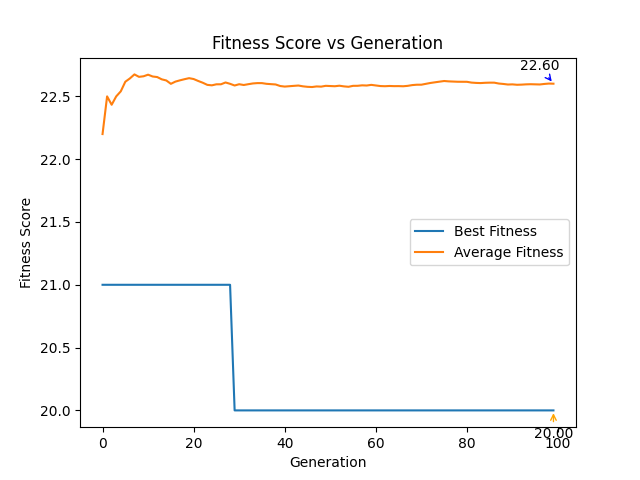
\includegraphics[width=0.475\textwidth]{../report/results/GCO_d2_a2_b4_g9.png}} \\ \hline
    \end{tabular}
    \caption{Alpha is lower than Beta ($ \alpha = 2.0, \beta = 4.0$)}
\end{figure}

When we kept $\alpha < \beta$, convergence was generally slower, even if the best was getting better, it was still really really slow. This is because the heuristics were given much more importance than the pheromone trail for the ants. So even when a good solution was found, it wasn't given much importance, thus the ants didn't always follow the better solution.

\textbf{Beta is Lower than Alpha}
\begin{figure}[H]
    \centering
    \begin{tabular}{| c | c |}
        \hline
        \subfloat[Dataset 1, Queen11]{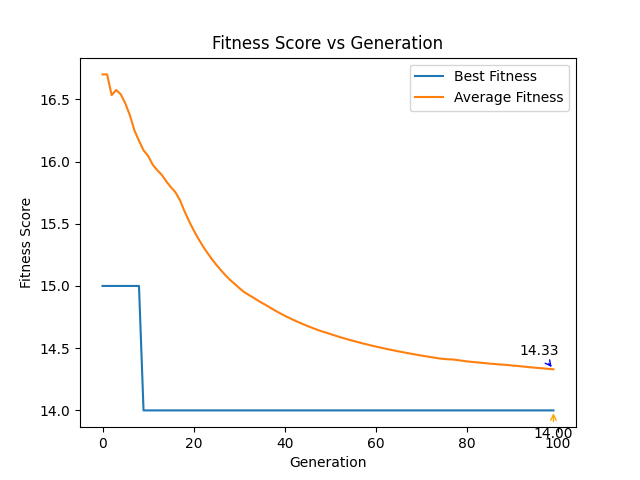
\includegraphics[width=0.475\textwidth]{../report/results/GCO_d1_a4_b2_g9.png}} & \subfloat[Dataset 2, le450]{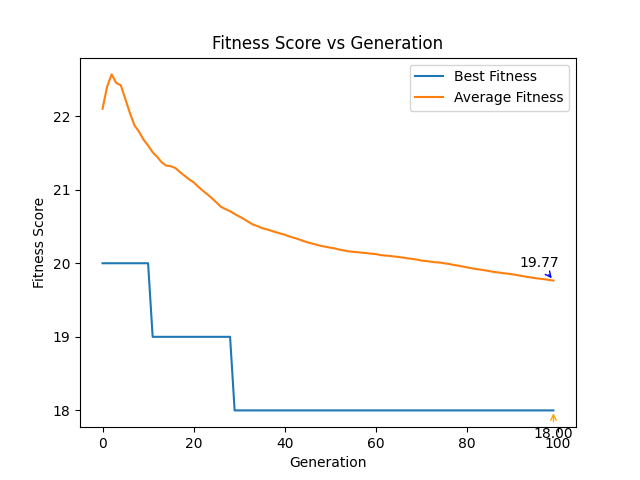
\includegraphics[width=0.475\textwidth]{../report/results/GCO_d2_a4_b2_g9.png}} \\ \hline
    \end{tabular}
    \caption{Beta is lower than Alpha ($ \alpha = 4.0, \beta = 2.0$)}
\end{figure}

When we kept $\beta < \alpha$, we started to see better results, as the ants started to prefer the pheromone trail over the heuristics. Then more ants eventually started to follow the better solution, thus, we can see not only some convergence as the average moves lower with increasing iterations, but also some better results in our best solution as well.

\textbf{Alpha and Beta are equal}
\begin{figure}[H]
    \centering
    \begin{tabular}{| c | c |}
        \hline
        \subfloat[Dataset 1, Queen11]{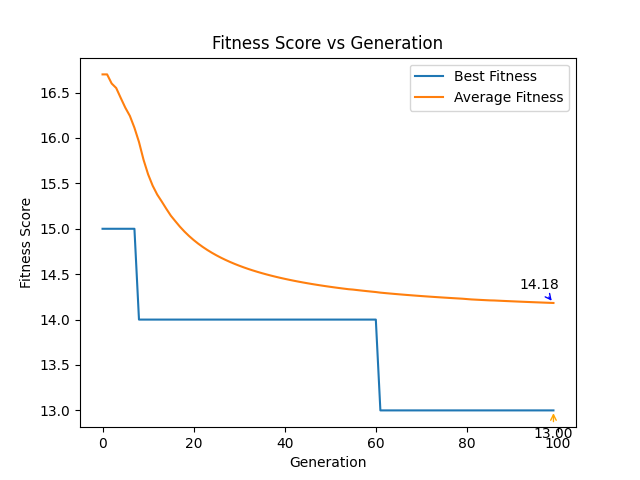
\includegraphics[width=0.475\textwidth]{../report/results/GCO_d1_a4_b4_g9.png}} & \subfloat[Dataset 2, le450]{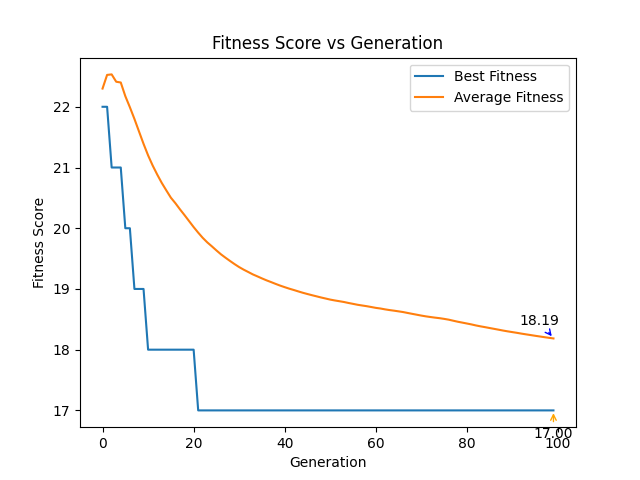
\includegraphics[width=0.475\textwidth]{../report/results/GCO_d2_a4_b4_g9.png}} \\ \hline
    \end{tabular}
    \caption{Alpha and Beta are equal($ \alpha = 4.0, \beta = 4.0$)}
\end{figure}

Now keeping $\alpha = \beta$, we see that the results are much better, since equal importance is given to both the pheromone trail and the heuristics. Then not only do the ants follow the better solution, but there is also an exploratory element of the search space. Thus, not only do we see that the average is going towards a convergence with the best solution, but also that the best solution is being optimized as well.

\textbf{Other Parameters}
\begin{itemize}
    \item Changing the value of $Q$, which is the amount of pheromones dropped by an ant, didn't really have much influence on our results. This is because the pheromones are updated after each ant has constructed a solution, and the pheromone trails are updated based on the quality of the solution. More pheromone is deposited on the color assignments that led to better solutions (i.e., colorings that used fewer colors). However, all in all, they are dropped in roughly the same proportion, and thus the results didn't change much.
    \item Changing the value of $\upgamma$ did infact have an influence on the results. Decreasing the value of $\upgamma$ lead to not only a slower convergence, but also increased chances of ants being stuck in a local optima, since there is a higher chance of pheromones being at any particular place even if it is not a good solution. Increasing the value of $\upgamma$ lead to a faster convergence, and also better results, since the pheromones were evaporating at a faster rate, and thus the ants were more likely to follow the better solution, since that was a shorter path and thus had more pheromones at any given time.
    \item Number of ants did have an impact on the results, since more ants meant more exploration of the search space, and thus a higher chance of finding a better solution. However, incresing the ants also lead to an increased time of computation, thus, the number of ants was kept between 10 and 20 for our implementation, as this was a good balance between the time of computation and the results.
    \item The number of iterations also had an impact on the results, since more iterations meant more exploration of the search space, and thus a higher chance of finding a better solution. However, incresing the iterations also lead to an increased time of computation, thus, the number of iterations was 100 for our implementation, as this was a good balance between the time of computation and the results.
\end{itemize}

\newpage
\subsubsection{Better Results}
Some of the better results have been shown below for each dataset.
\begin{figure}[H]
    \centering
    \begin{tabular}{| c | c |}
        \hline
        \subfloat[Best for Dataset1 (5k Iters) Heuristic 1]{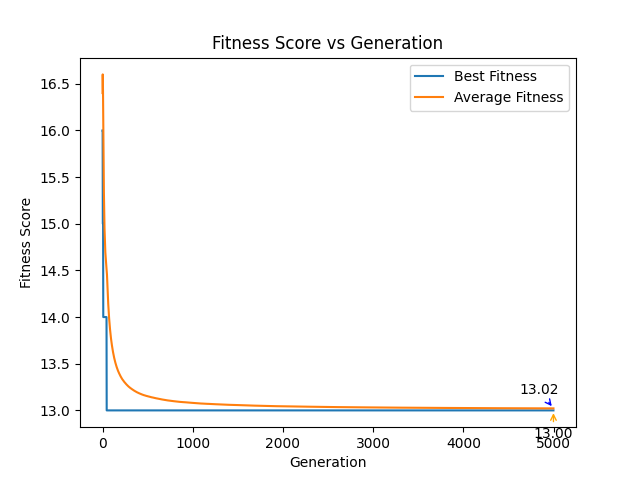
\includegraphics[width=0.45\textwidth]{../report/results/GCO_d1_5k_convergence.png}} & \subfloat[Convergence for Dataset1 (2k Iters) Heuristic 1]{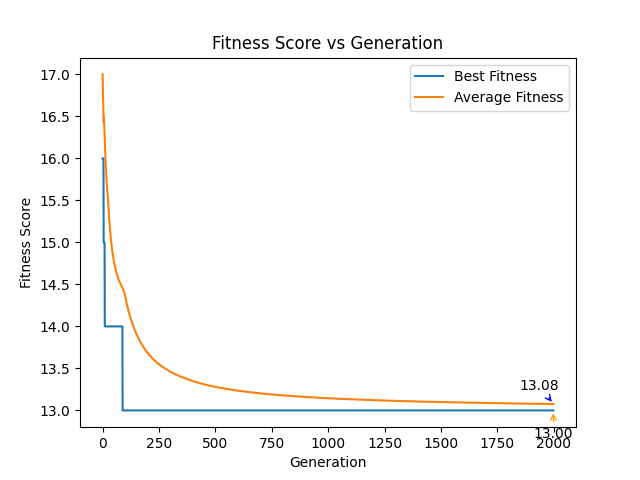
\includegraphics[width=0.45\textwidth]{../report/results/GCO_d1_2000itesrs.png}}  \\ \hline
        \subfloat[Convergence for Dataset1 - Heuristic 3]{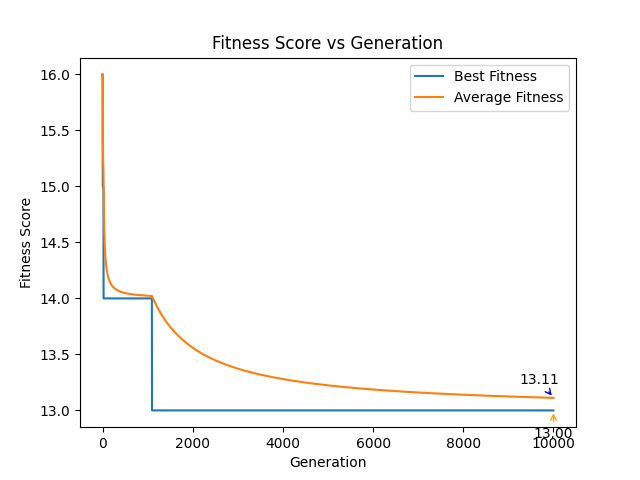
\includegraphics[width=0.45\textwidth]{../report/results/GCO_d1_convergence_10k_h3.png}} & \subfloat[Best for Dataset2]{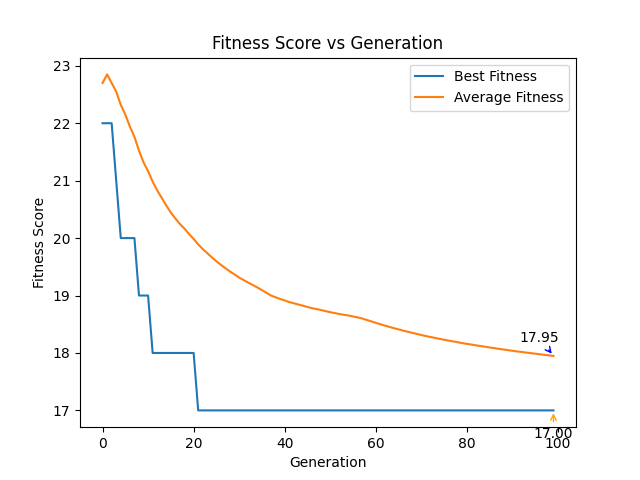
\includegraphics[width=0.45\textwidth]{../report/results/GCO_d2_h3_best.png}} \\ \hline
        \subfloat[Near Convergence Dataset2 - Heuristic 3]{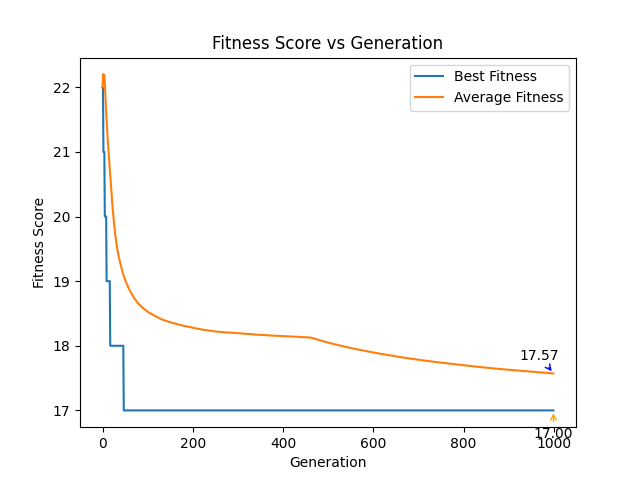
\includegraphics[width=0.45\textwidth]{../report/results/GCO_d2_nearconv.png}} & \subfloat[Near Convergence Dataset2 - Heuristic 3]{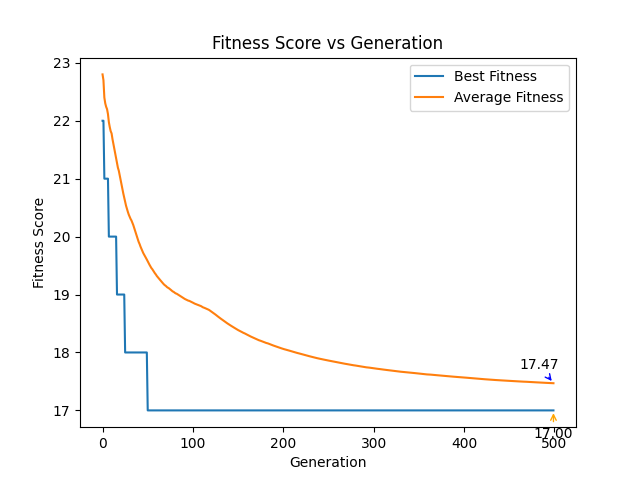
\includegraphics[width=0.45\textwidth]{../report/results/GCO_d2_conv.png}} \\ \hline
    \end{tabular}
\end{figure}

% \begin{figure}[H]
%     \centering
%     \begin{tabular}{| c | c |}
%         \hline
%         \subfloat[Dataset 1, Queen11]{\includegraphics[width=0.475\textwidth]{../report/results/}} & \subfloat[Dataset 2, le450]{\includegraphics[width=0.475\textwidth]{../report/results/}} \\ \hline
%     \end{tabular}
%     \caption{}
% \end{figure}

% \bibliographystyle{9}
\section{References}
\begin{thebibliography}{9}
    \bibitem{Paper} \hypertarget{refpaper}{} Bessedik, Malika \& Laib, R. \& Boulmerka, Aissa \& Drias, Habiba. (2005). Ant Colony System for Graph Coloring Problem. 786- 791. 10.1109/CIMCA.2005.1631360.
    \bibitem{RLF} \hypertarget{rlfmethod}{} Daniel Brélaz. 1979. New methods to color the vertices of a graph. Commun. ACM 22, 4 (April 1979), 251-256. \href{https://doi.org/10.1145/359094.359101}{https://doi.org/10.1145/359094.359101}
\end{thebibliography}
\end{document}
